\subsection{Workload Distribution Study}
\label{subsec:workload-distribution-study}

The workload distribution study focuses on analyzing the impact of different scheduling strategies on parallel performance. This experiment evaluates the runtime and speedup for static and dynamic scheduling methods across thread counts of 1, 2, 4, 8, 16, 32, 64, 128, and 256. The configurations include static scheduling, dynamic scheduling with a chunk size of 1 (\texttt{dynamic-1}), and dynamic scheduling with a chunk size of 16 (\texttt{dynamic-16}).

For lower thread counts (2, 4, and 8), both \texttt{dynamic-1} and \texttt{dynamic-16} outperform static scheduling, as shown in Figure~\ref{fig:load-imbalance-speedup}. The dynamic approaches provide better load balancing, reducing runtime compared to the static method. However, as the thread count increases beyond 8, the performance of static scheduling converges with that of \texttt{dynamic-1}, with static even slightly outperforming \texttt{dynamic-1} at higher thread counts. This performance crossover is attributed to reduced scheduling overhead in static scheduling when many threads are utilized.

Dynamic scheduling consistently outperforms static scheduling, but the performance gap becomes significant with a thread count of 256. Specifically, \texttt{dynamic-1} achieves a speedup of 21.8 times, compared to 18.9 times for static scheduling. The large disparity is attributable to the limited height of the image (288 pixels), which constrains the number of iterations being parallelized by static scheduling. 

As shown in the \texttt{ray\_color} function in Listing~\ref{listing:ray-color}, simulating the ray color for the sky region is relatively computationally light. When a ray does not intersect any objects in the scene, no recursion is necessary, significantly reducing the computational workload for these regions. Furthermore, as shown in Figure~\ref{fig:sample-image-fine}, the upper part of the image generated in our testing is largely sky without objects, making the static scheduling inefficient due to the uneven workload distribution.

These findings indicate that while dynamic scheduling is effective for addressing load imbalance, the choice of chunk size and the problem size significantly influence performance. Future studies should explore configurations with larger workloads and higher scene complexity to better utilize the available computational resources.

\begin{figure}[htbp]
    \centering
    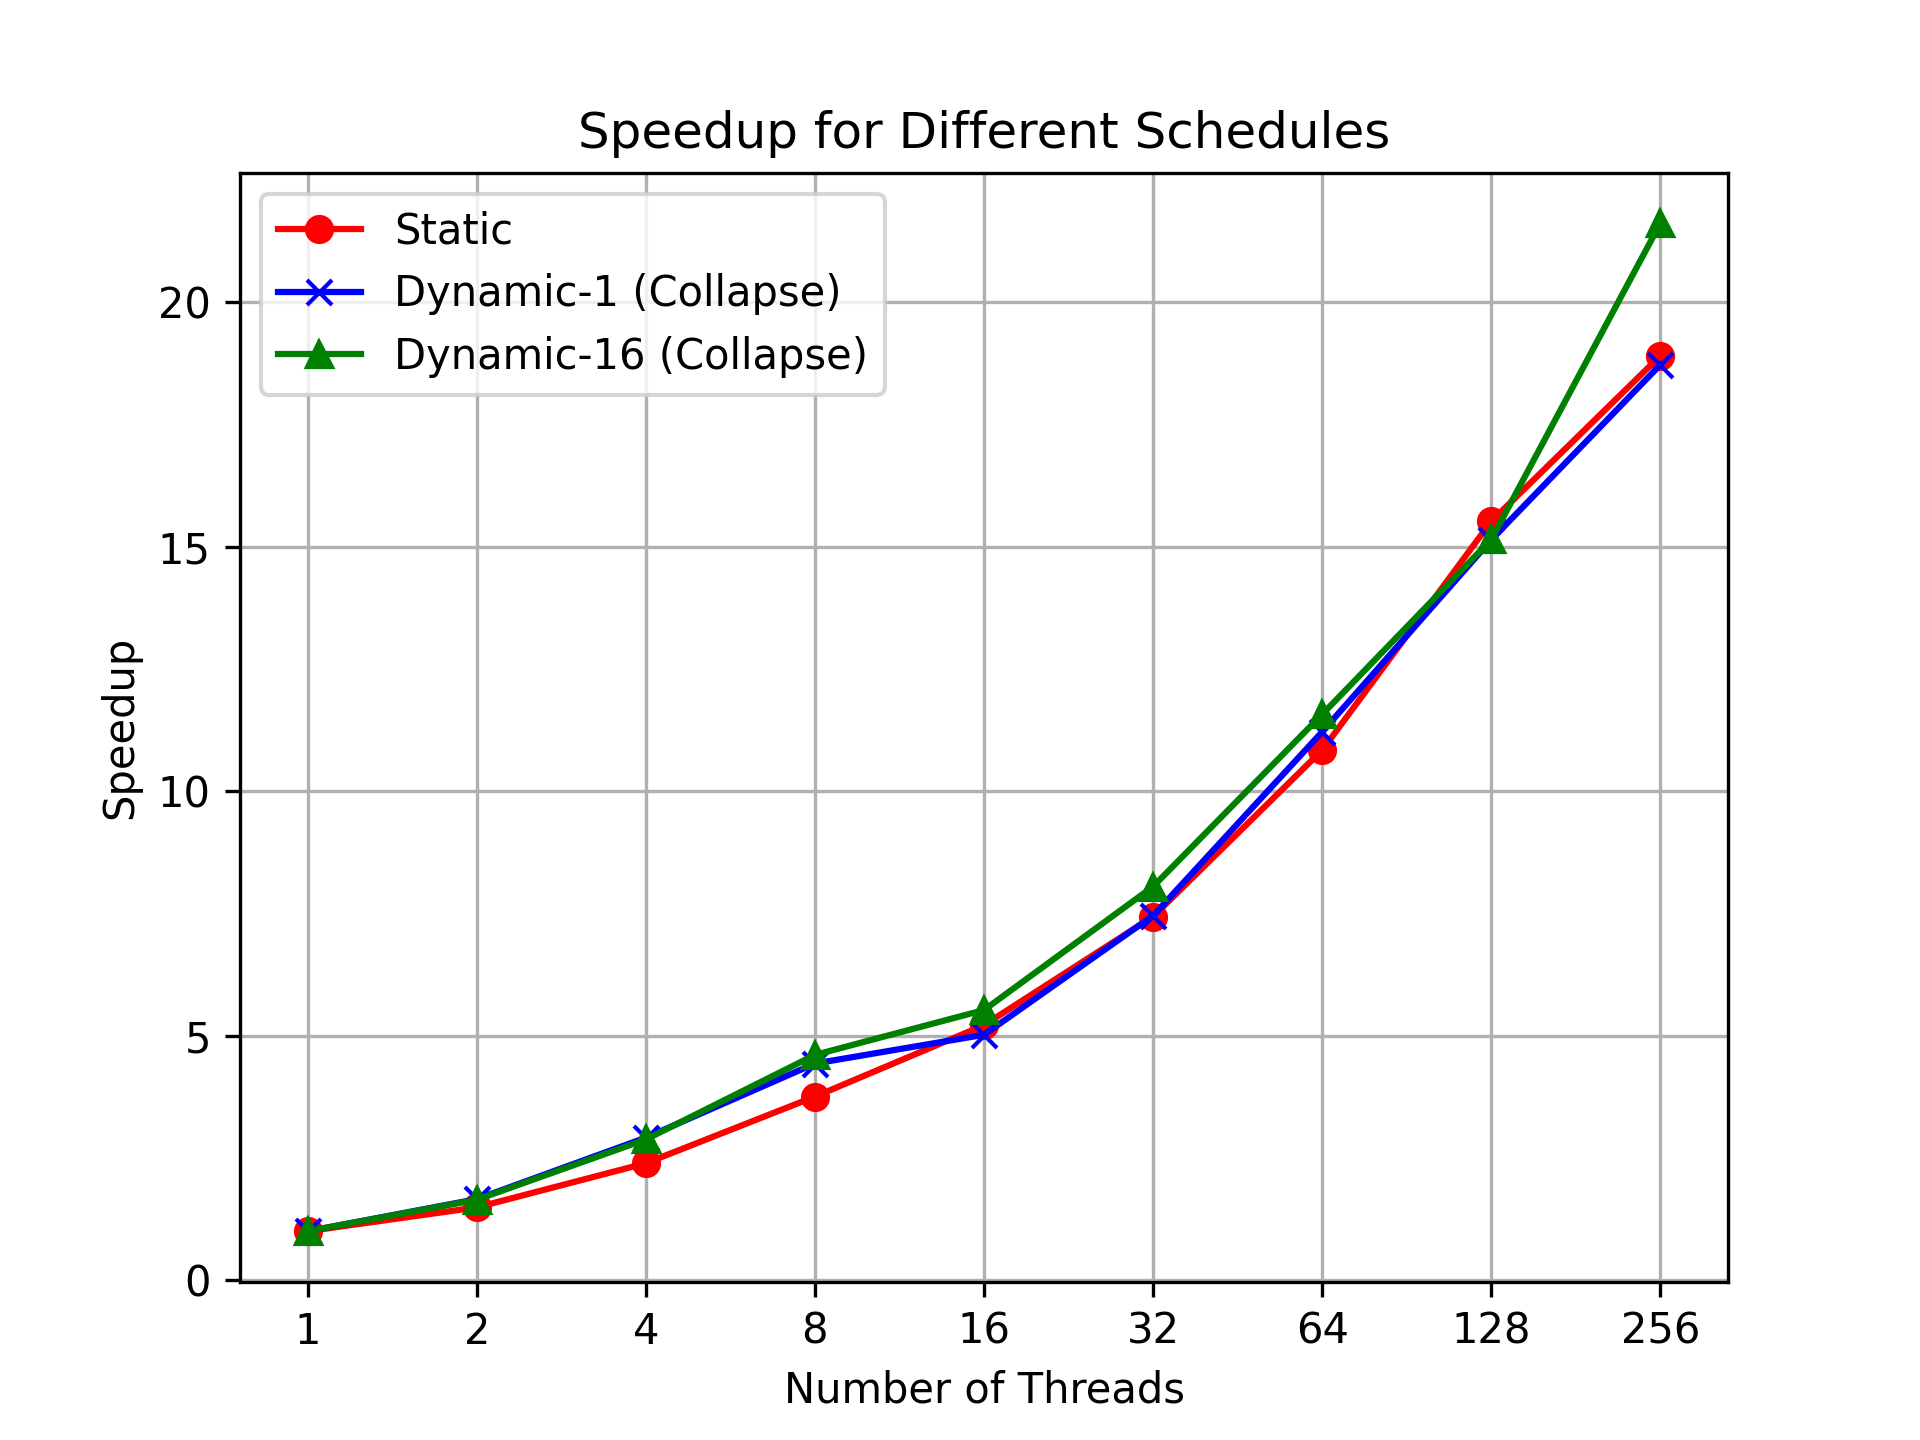
\includegraphics[width=1.0\linewidth]{images/load_imbalance_speedup_comparison.png}
    \caption{Comparison of speedup across different scheduling strategies (static and dynamic) with varying chunk sizes. The results highlight the trade-offs between load balancing and scheduling overhead.}
    \label{fig:load-imbalance-speedup}
\end{figure}